\documentclass{article}
\usepackage{amsmath, amssymb}
\usepackage{graphicx}
\usepackage{hyperref}

\title{Mathematical Techniques in WAV Analysis and Note Detection}
\author{}
\date{}

\begin{document}

\maketitle

\section{Introduction}
This report outlines the mathematical techniques considered, implemented, and utilized in the final version of our WAV analysis project. The project aimed to robustly determine note durations and generate MusicXML, with an ultimate goal of creating PDF sheet music. Our primary approach to pitch detection was autocorrelation, while note onsets were determined using both peak detection in energy and spectral energy differences derived from the Short-Time Fourier Transform (STFT).

\section{Techniques Utilized in the Final Project}
These mathematical methods were actively employed in the final implementation:

\subsection{Mono Conversion via Stereo Averaging}
Since WAV files may contain stereo channels, we converted them to mono by averaging the left and right channels, ensuring a unified signal for processing.

\subsubsection{How Stereo Averaging Works}
Stereo signals contain two independent channels, often representing left and right audio. To process them as a single signal, we compute their average:

\begin{equation}
x_{mono}(n) = \frac{x_{left}(n) + x_{right}(n)}{2}
\end{equation}

This preserves the overall amplitude structure while ensuring consistency in pitch detection and onset analysis.

\begin{figure}[h]
\rotatebox[origin=c]{180}{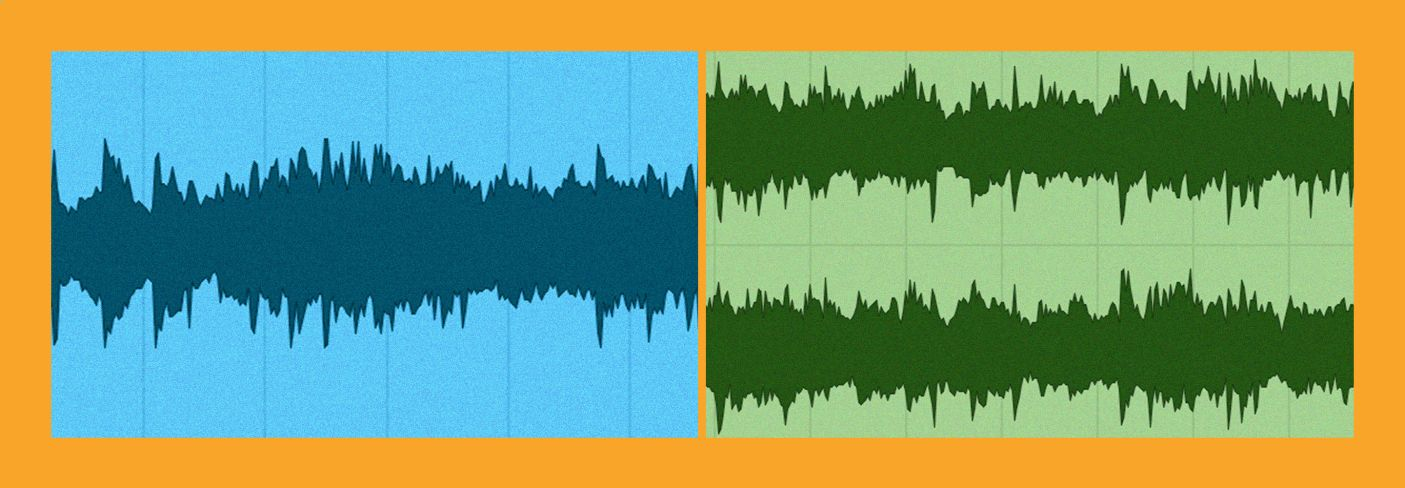
\includegraphics[width=125mm,scale=0.5]{docs/Research Report/Stereo-To-Mono.jpg}}
\caption{Conversion of Stereo Audio to Mono-Audio by averaging channels$^1$}
\end{figure}

\newpage

\subsection{Autocorrelation for Pitch Detection}
Autocorrelation was used to determine the fundamental frequency of the audio signal by analyzing periodic patterns. This method proved effective for identifying stable pitches but had limitations when dealing with fast note transitions.

\subsubsection{How Autocorrelation Works}
Autocorrelation is a time-domain signal processing technique used to detect periodicity in a signal. It involves multiplying a signal by a time-shifted version of itself and summing the result over all possible shifts. The resulting function exhibits peaks at integer multiples of the signal's fundamental period, allowing the estimation of the dominant frequency. This method is particularly useful in pitch detection, as musical notes exhibit periodic waveforms.

Mathematically, the autocorrelation function $R(\tau)$ of a discrete signal $x[n]$ is defined as:

\begin{equation}
R(\tau) = \sum_{n=0}^{N-1} x[n] x[n+\tau]
\end{equation}

where $\tau$ represents the lag and $N$ is the signal length.

\begin{figure}[h]
    \centering
    \begin{tabular}{ccc}
        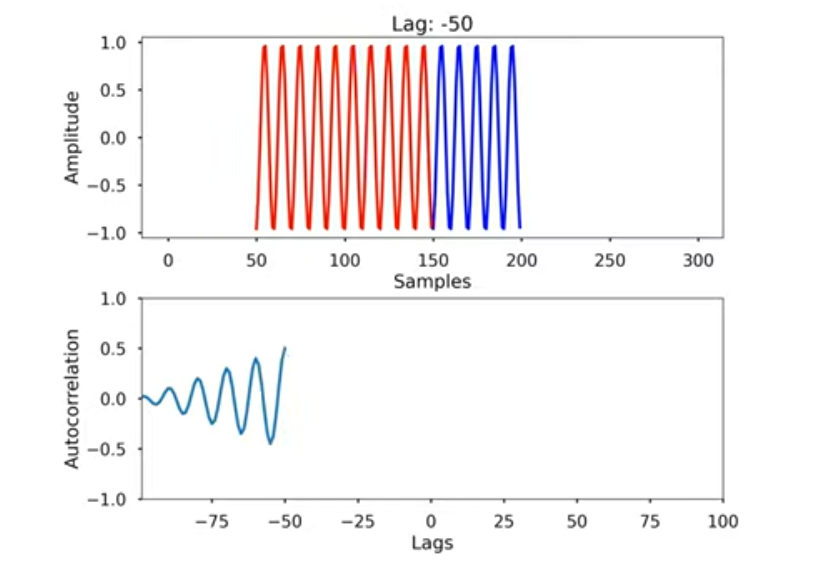
\includegraphics[width=60mm]{docs/Research Report/autocorrelation.png} & 
        $\Longrightarrow$ & 
        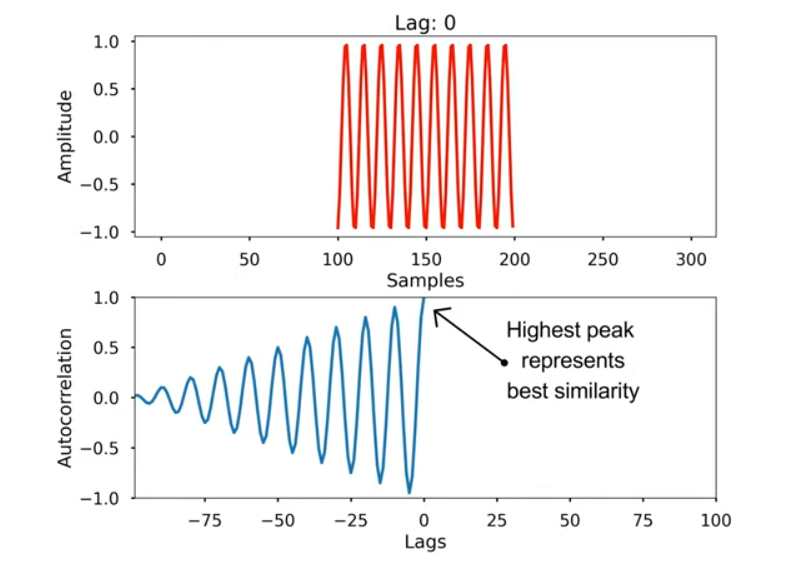
\includegraphics[width=60mm]{docs/Research Report/autocorrelation Peak.png} \\
    \end{tabular}
    \caption{Signal peak occurs when offset signal is most similar to original signal$^2$}
    \label{fig:autocorrelation_peak}
\end{figure}

\newpage

\subsection{Peak Detection in Energy for Note Onsets}
By tracking changes in energy levels over time, we detected note onsets. Peaks in energy served as markers for the start of new notes, a fundamental aspect of transcription.

\subsubsection{How Peak Detection Works}
Peak detection involves identifying significant local maxima in a signal. This is commonly done by analyzing the derivative of an energy envelope and applying a threshold-based criterion to filter out minor fluctuations. The energy envelope can be computed using the root mean square (RMS) or the sum of squared amplitudes within a short sliding window.

Mathematically, energy $E(n)$ of a signal in a window of length $M$ is given by:

\begin{equation}
E(n) = \sum_{m=0}^{M-1} x^2[n-m]
\end{equation}

Peak detection then involves identifying points where $E(n)$ surpasses an adaptive threshold.

\subsection{STFT for Spectral Analysis and Onset Detection}
We employed a Short-Time Fourier Transform (STFT) to generate spectrograms and analyze spectral energy changes. Differences in spectral energy were used as an alternative onset detection method, complementing the energy peak detection approach.

\subsubsection{How STFT Works}
The STFT is a method of analyzing the frequency content of a signal over time by applying the Fourier Transform to short, overlapping segments of the signal. It provides a time-frequency representation, allowing the observation of spectral variations that correspond to note onsets.

Mathematically, the STFT of a signal $x(t)$ with a window function $w(t)$ is defined as:

\begin{equation}
X(t, f) = \int_{-\infty}^{\infty} x(\tau) w(\tau - t) e^{-j 2\pi f \tau} d\tau
\end{equation}

where $w(t)$ is typically a Hanning or Hamming window to reduce spectral leakage.

\begin{figure}[h]
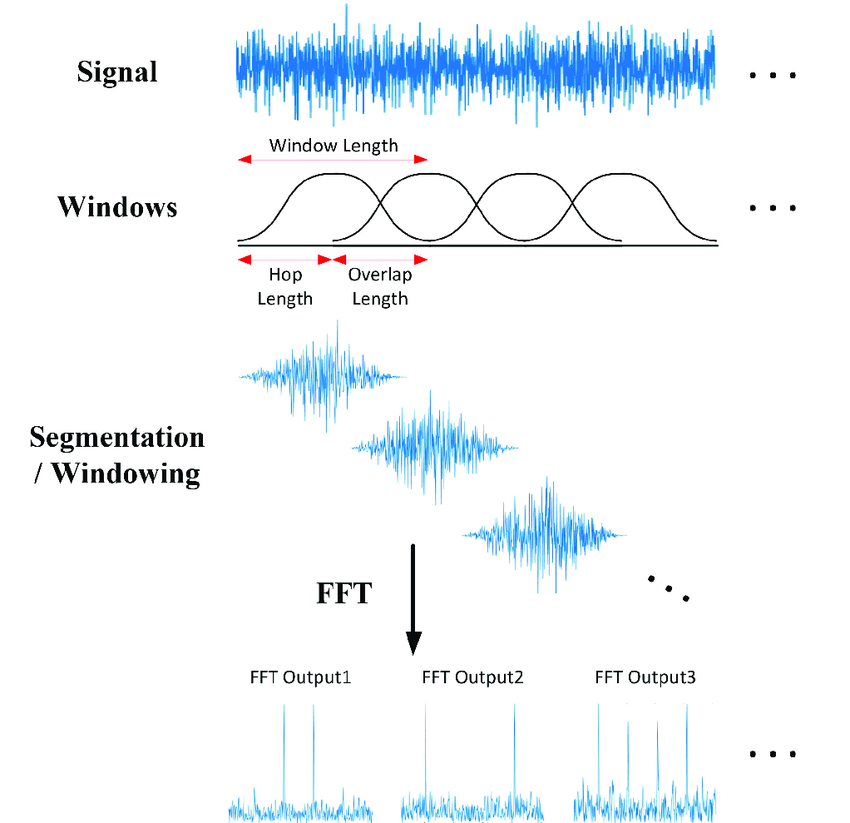
\includegraphics[width=125mm,scale=0.5]{docs/Research Report/STFT.png}
\caption{Breakdown of STFT Process used to construct spectrogram$^3$}
\end{figure}

\newpage

\subsection{Hanning Window}
Both Hanning and Hamming windows were tested as potential smoothing functions for spectral analysis. They were used in different configurations of STFT, though ultimately, the Hanning functino was chosen based on performance.

\subsubsection{How Windowing Functions Work}
Window functions taper the edges of a signal segment before applying Fourier analysis, reducing spectral leakage. The Hanning window is defined as:

\begin{equation}
w(n) = 0.5 - 0.5\cos\left(\frac{2\pi n}{N-1}\right)
\end{equation}

\begin{figure}[h]
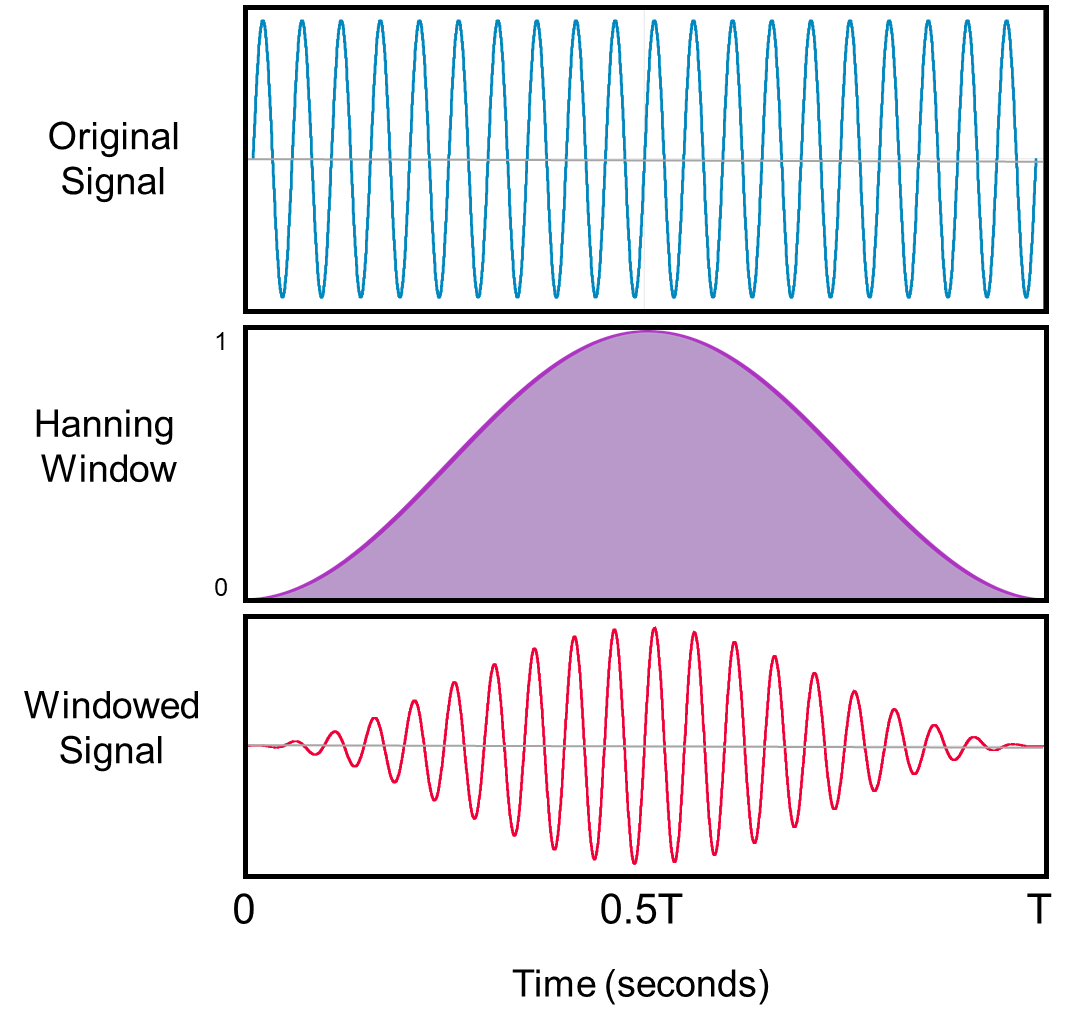
\includegraphics[width=125mm,scale=0.5]{docs/Research Report/hanning.png}
\caption{Hanning function used to smooth out signal onsets$^4$}
\end{figure}

\newpage

\subsection{Krumhansl-Schmuckler Key-Finding Algorithm}
This algorithm was used for determining the key signature of a musical piece based on pitch class profiles 

\subsubsection{How the Key-Finding Algorithm Works}
The Krumhansl-Schmuckler algorithm matches pitch distributions in an audio signal to predefined key profiles, computing a correlation score for each possible key. The key with the highest correlation is selected.

\begin{figure}[h]
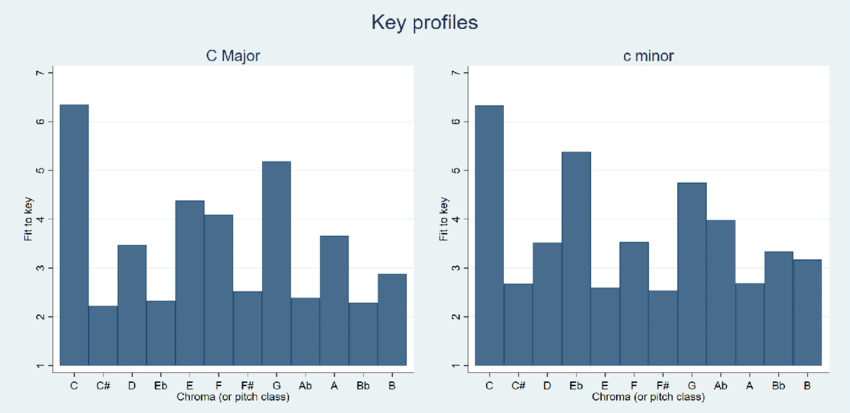
\includegraphics[width=125mm,scale=0.5]{docs/Research Report/C-Cminor-Expected-Key-Profiles.png}
\caption{Expected Relative Note Frequency profiles of C and C-Minor key, used in Krumhansl-Schmukler algorithm to create correlation scores$^5$}
\end{figure}

\newpage

\section{Techniques Considered but Not Implemented}
Several mathematical techniques were considered but ultimately not implemented in any phase of development.

\subsection{Cross-Correlation}
Cross-correlation was evaluated as a potential enhancement for pitch detection and time-domain alignment.

\subsubsection{Mathematical Definition}
Given two signals $x(t)$ and $y(t)$, their cross-correlation is defined as:
\begin{equation}
(R_{xy} \ast x)(\tau) = \int_{-\infty}^{\infty} x(t) y(t + \tau) dt.
\end{equation}
This operation measures the similarity of $x(t)$ and a time-shifted version of $y(t)$. In the discrete case, for signals sampled at intervals $n$, it is given by:
\begin{equation}
R_{xy}[k] = \sum_{n} x[n] y[n+k].
\end{equation}
Cross-correlation is extensively used in time-delay estimation and pattern recognition. The Fast Fourier Transform (FFT) can accelerate its computation through:
\begin{equation}
R_{xy} = \mathcal{F}^{-1} \{ X^*(f) Y(f) \},
\end{equation}
where $X(f)$ and $Y(f)$ are the Fourier transforms of $x(t)$ and $y(t)$, and $X^*(f)$ is the complex conjugate of $X(f)$. \\

\textbf{Could have been used for} improved time alignment of detected note events, reducing timing inaccuracies in sheet music generation.

\begin{figure}[h]
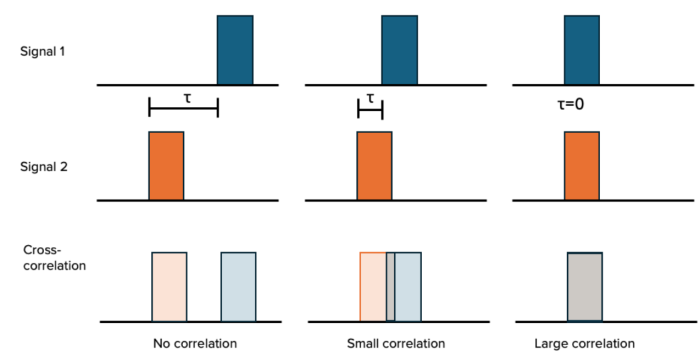
\includegraphics[width=125mm,scale=0.5]{docs/Research Report/cross-correlation-example.png}
\caption{Diagram highlighting Cross-Correlation functionality. Similar to Auto-correlation but used for different signals, rather than offsets of same signal$^6$}
\end{figure}

\newpage

\subsection{Wavelet Denoising}
Wavelet denoising is a signal processing technique that uses wavelet transforms to separate a signal into different frequency components and apply thresholding to reduce noise. It is particularly effective for denoising non-stationary signals, such as audio, where the noise is typically localized in time or frequency.

\subsubsection{How Wavelet Denoising Works}
Wavelet denoising involves three main steps:  \\

1. \textbf{Wavelet Transform}: The signal is decomposed into a series of wavelet coefficients using a discrete wavelet transform (DWT) or continuous wavelet transform (CWT). The DWT splits the signal into \textbf{approximation} coefficients (low frequencies) and \textbf{detail} coefficients (high frequencies) at multiple scales.
   
   Mathematically, the DWT of a signal \( x(t) \) is represented as:
   \[
   x(t) = \sum_{j} \sum_{k} c_{jk} \psi_{jk}(t)
   \]
   where \( \psi_{jk}(t) \) are the wavelet functions at scale \( j \) and position \( k \), and \( c_{jk} \) are the wavelet coefficients. \\

2. \textbf{Thresholding}: The wavelet coefficients corresponding to the high-frequency noise are identified and thresholded. The thresholding technique reduces or removes coefficients that correspond to noise while preserving those that correspond to signal features. There are two types of thresholding: \\
   - \textbf{Hard Thresholding}: Coefficients smaller than a set threshold are set to zero. \\
   - \textbf{Soft Thresholding}: Coefficients smaller than a threshold are shrunk towards zero, reducing the magnitude of the larger coefficients while eliminating smaller ones. \\

   Mathematically, soft thresholding is given by:
   \[
   \hat{c}_{jk} = \text{sign}(c_{jk}) \cdot \max(0, |c_{jk}| - \lambda)
   \]
   where \( \lambda \) is the threshold value. \\

3. \textbf{Inverse Wavelet Transform}: After thresholding, the signal is reconstructed by applying the inverse wavelet transform, which combines the modified coefficients back into the time domain to produce the denoised signal.

\subsubsection{Advantages of Wavelet Denoising}
- Wavelet denoising is highly effective at removing localized, high-frequency noise while preserving important signal features like sharp transients, which is important for tasks like music transcription.
- The method can be adapted to different levels of noise by adjusting the thresholding parameters and using different wavelet functions for specific types of signals. \\

\textbf{Could have been used for} denoising input audio, effectively reducing high-frequency noise that could interfere with accurate note onset detection and improving the clarity of secondary notes for transcription.

\begin{figure}[h]
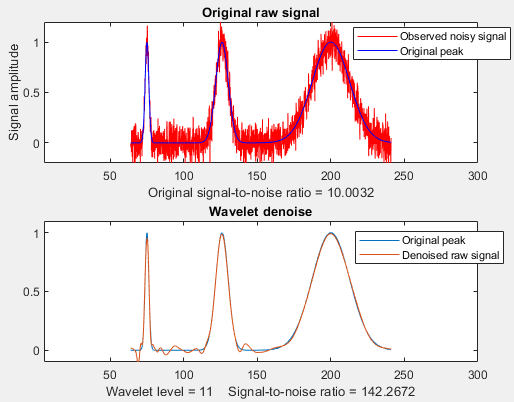
\includegraphics[width=125mm,scale=0.5]{docs/Research Report/denoise-filter.png}
\caption{ Signal Denoising via soft wavelet thresholding$^7$}
\end{figure}

\newpage



\subsection{Yin Algorithm for Pitch Detection}
The Yin algorithm, a robust pitch detection technique, was considered.

\subsubsection{Mathematical Basis}
Yin refines autocorrelation by computing a difference function:
\begin{equation}
d(\tau) = \sum_{t=1}^{T} (x_t - x_{t+\tau})^2.
\end{equation}
A cumulative mean normalization step is then applied:
\begin{equation}
\tilde{d}(\tau) = d(\tau) / \left(\frac{1}{\tau} \sum_{j=1}^{\tau} d(j) \right).
\end{equation}
Pitch corresponds to the minimum of $\tilde{d}(\tau)$. This improves over standard autocorrelation by reducing octave errors and improving resolution at low frequencies. \\

\textbf{Could have been used to} refine pitch estimation, reducing frequency detection errors and improving note transcription accuracy.

\begin{figure}[h]
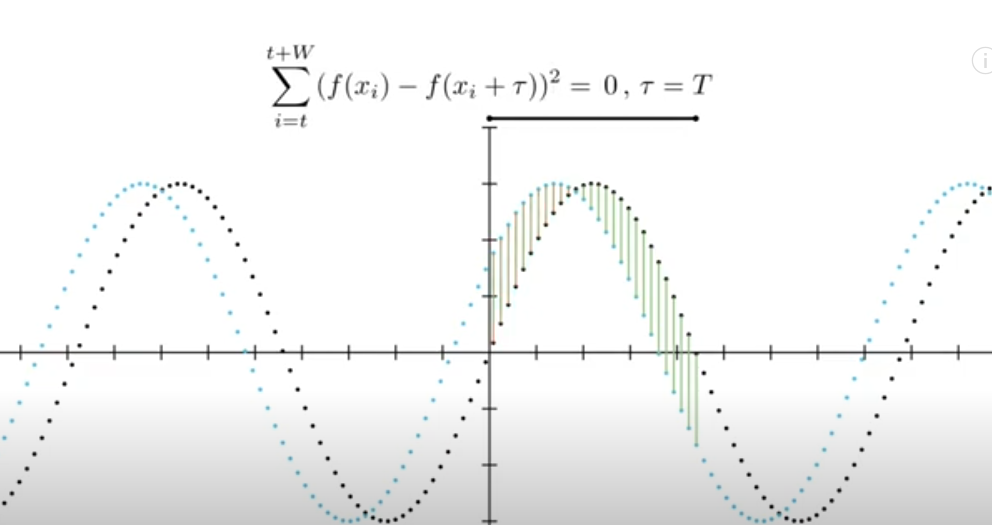
\includegraphics[width=125mm,scale=0.5]{docs/Research Report/yin-function.png}
\caption{Difference in signal offsets calculated to determine cumulative mean difference, allowing better handling of noisy inputs or harmonics$^8$}
\end{figure}

\newpage


\section{Conclusion}
This project employed a combination of signal processing techniques to achieve accurate pitch detection and onset analysis. While several methods were considered, the final implementation balanced computational efficiency with accuracy. Future improvements could explore more advanced onset detection mechanisms and integrate additional filtering techniques to refine transcription accuracy.


\newpage
\begin{thebibliography}{9}

\bibitem{iZotope}
iZotope. (n.d.). \textit{Mono vs. stereo in audio mixing}. Retrieved from \url{https://www.izotope.com/en/learn/mono-vs-stereo.html}

\bibitem{YouTube1}
YouTube. (n.d.). \textit{YouTube}. Retrieved from \url{https://www.youtube.com/watch?v=uf679Qo-bB4}

\bibitem{STFT}
Figure 1. (n.d.). \textit{Short-time Fourier transform (STFT) overview}. Retrieved from \url{https://www.researchgate.net/figure/Short-time-Fourier-transform-STFT-overview_fig1_346243843}

\bibitem{Siemens}
Siemens Digital Industries Software Community. (n.d.). Retrieved from \url{https://community.sw.siemens.com/s/article/Overlap-What-Why-and-How-to-use-it}

\bibitem{TonalStructure}
Empirical Musicology Review. (n.d.). \textit{Tonal and “Anti-Tonal” Cognitive Structure in Viennese Twelve-Tone Rows}. Retrieved from \url{https://ojs.library.osu.edu/index.php/EMR/article/view/7655/5748}

\bibitem{CrossCorrelation}
Jball. (2025, February 4). \textit{What is cross-correlation, and how does it advance spectrum analysis?}. Liquid Instruments. Retrieved from \url{https://liquidinstruments.com/blog/cross-correlation-and-spectrum-analysis/}

\bibitem{Wavelets}
Intro. to Signal Processing. (n.d.). \textit{Wavelets and wavelet denoising}. Retrieved from \url{https://terpconnect.umd.edu/~toh/spectrum/wavelets.html}

\bibitem{YouTube2}
YouTube. (n.d.-a). \textit{YouTube}. Retrieved from \url{https://www.youtube.com/watch?app=desktop&v=W585xR3bjLM}

\end{thebibliography}

\end{document}

